\secspace

\section{Protecting Video Imagery with \system{}}
\label{sec:method}
We have identified that video imagery is susceptible to style mimicry attacks
despite existing protection in image space (\S\ref{sec:eval-limitations}).
Although current protection tools are effective for 2D art, they are no longer robust
to adaptive adversaries in the video domain. In this section, we
develop \system, a framework that extends image-based protection tools to the video
domain, resulting in improved robustness against adaptive adversaries as well
as lower computation costs and improved video quality for protected videos.

\begin{table}[t]
  \centering
    \resizebox{0.4\textwidth}{!}{
    \centering
\begin{tabular}{c|cc}
  Protection Tool & Protected        & Protected + Pixel Averaging                 \\ \hline
  Glaze          & 70.59 $\pm$ 1.05 & \textbf{23.76 $\pm$ 1.14} \\
  Mist           & 62.90 $\pm$ 1.11 & \textbf{25.34 $\pm$ 1.14} \\
  Anti-DB        & 59.28 $\pm$ 1.18 & \textbf{22.62 $\pm$ 1.15} 
  \end{tabular}}
  \caption{Human feedback (Protection Success Rate) shows perturbation
    removal can significantly reduce effects of protection tools 
    against style mimicry attacks. Note baseline PSR for original,
    unprotected frames is 17.65 $\pm$ 1.10.}
\label{tab:user-study-removal-results}
\vspace{-0.2in}
\end{table}

\begin{figure*}[t]
  \centering
  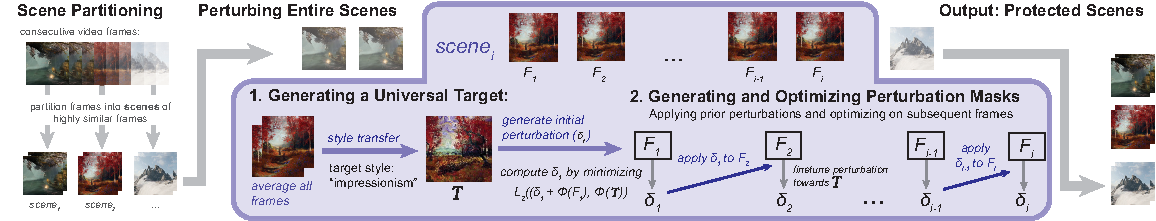
\includegraphics[width=1\textwidth]{plots/system-design-02-eps-converted-to.pdf}
  \vspace{-0.25in}
  \caption{\system~ partitions videos into scenes by measuring average pixel difference. Each scene is perturbed using a two-part process: 1) A target image ($T$) is computed by averaging all frames and style transferring to a 'target style' 2) Perturbations are iteratively applied and optimized by minimizing latent $L_2$ norm between $T$ and the perturbed frame.}
  \label{fig:system-design}
\end{figure*}


\subsection{Design intuition} 

\para{Challenges of existing perturbation systems.} Existing perturbation
systems do not take into account the threat of an adversary gaining access to
highly similar or even identical frames that are protected with completely
independent perturbations.  These systems independently optimize separate
protection perturbations for each frame.

This optimization process includes 1) generating a \textit{random} target latent
tensor, and 2) perturbing the original image by optimizing the 
image towards the selected target.  The choice of target significantly
impacts the pixel level perturbations on an image. Current systems choose
targets by generating a latent representation of the original image,
introducing noise, and then employing denoising autoencoders.  This
randomness (\ie non-linearity) is desired for image-based protection, making
it more challenging to reverse engineer or remove the perturbations. However,
it also leads to each perturbation mask being entirely unique; disregarding
the temporal redundancy present in the original frames. This in turn gives
rise to effective countermeasures that remove the protection
(\S\ref{sec:eval-limitations}).

\para{Intuition.}
Our key intuition is that if we can create very similar perturbations on
similar underlying frames, we can nullify the adversaries ability to exploit
duplicity in frames. With this in mind, there are two simple options for
perturbing a scene of similar frames. The first option is to re-use the same
perturbation for the entire scene. Re-using the same perturbation is robust
to pixel averaging attacks, but frame-specific protection weakens after
small levels of movement in frames.

A second option is that if we can chose very similar targets (that guide the
optimizing of perturbations) for similar frames, we can increase the
consistency between perturbations. We find that re-using a single target
tensor throughout a scene leads to very similar perturbations, but also makes
frames less robust to style mimicry. This is because the perturbation
optimization algorithm is not able to customize the embeddings of different
frames to the same degree as it does for the original frame the
target tensor was generated from. Thus our goal is to 1) divide 
videos into scenes that can share a \textit{universal} target, 2) generate
this ``universal target'' for each scene, and 3) optimize perturbations on
subsequent frame to maximize protection against mimicry.

\subsection{System Design}

Figure~\ref{fig:system-design} describes our pipeline for generating robust,
protected videos by partitioning them into scenes, generating a target image
for each scene, and then optimizing the perturbations on each frame towards
its respective target. 

\para{Scene partitioning.}  We want to pinpoint sections of videos where
using different perturbations might leave frames vulnerable to averaging
attacks. We split videos into distinct scenes based on frame similarity, and
considered existing scene partitioning algorithms and
tools~\cite{pyscenedetect}. Note that we require all frames in a scene to be
similar enough to share a single ``perturbation target.'' This is a stronger
constraint than most prior definitions for a ``scene,'' leading us to
implement our own algorithm. We split scenes based on the mean pixel
difference between two consecutive frames $F_i$ and $F_{i-1}$, defined
by \secspace
\begin{equation}
 \frac{Pixel(F_i, F_{i-1})}{N}< \epsilon_{scene}\label{eq:mean_pixel_diff}
\end{equation}
where $N$ is the number of pixels per frame and $Pixel(.)$ calculates
the pixel difference between two frames, and $\epsilon_{scene}$ is a
parameter for scene partition. 

\para{Generating a universal target.}  To create consistency between
consecutive perturbations, we compute a single target image for all frames in
a scene. This means that the target embedding needs to be close enough the
embeddings of each frame in the scene, so that it can correctly guide each
individual optimization. We test several approaches to generating the target
tensor: 1) using the middle frame from the scene as base image, 2) generating
image embeddings of each frame in the scene, calculating the centroid of
these embeddings as base image, and 3) averaging all frames together as base
image. We measure latent $L_2$ norm distance between the embedding of each unique frame in a
scene and the target tensor, and find that averaging all frames in a scene
leads to a target that is consistently the closest distance across all frames
(Figure~\ref{fig:target-selection-algorithm-results} in Appendix).

Specifically, we compute a style transferred target image $T$ from the averaged
image, like prior work~\cite{shan2023glaze}. We select a video-specific
prompt to guide the style transfer, for example: \textit{Japanese Anime} videos
use ``impressionist painting by Van Gogh'' as the target style.

\para{Generating and optimizing perturbation masks.}  We consider several
factors when computing perturbations: maximizing protection, robustness
against perturbation removal attacks, and finally, reducing computation
costs. We balance re-using perturbations on subsequent frames \textit{which
  enhances robustness against removal attacks} with optimizing or recomputing
perturbations \textit{which maintains high protection levels against mimicry
  attacks}. Protection success is achieved by reducing loss between a
perturbed image and target image. We develop our algorithm for perturbing a
scene as follows:

\if 0

\begin{packed_itemize}
  \item We compute $T_s$ using all frames in a scene (described above).
  \item The first frame $F_1$ is perturbed normally, optimizing towards
    $T_s$.
  \item For following frames, we first consider the current perturbation mask.
  If we measure the distance $L_2(F_2,T_s)$ and 
  is close enough to $L_2(F_1,T_s)$, we allow reusing perturbation on this
  frame. If not close enough, we continue optimization process on the reused
  perturbation for $F_2$ until loss decreases enough. Alternatively, if loss
  surpasses our second threshold we recompute perturbation fully. Because the
  perturbation is generated using the same target image, the system maintains
  high consistency between perturbations.
\item Repeat this process for each consecutive frame in order, using the
  latest updated perturbation mask as the base.
\end{packed_itemize}

\fi

\begin{packed_itemize}
  \item Given the current scene and its corresponding $M$ frames $\{F_i\}_{i=1}^{M}$, compute the target frame $T$ (described above).
  \item For the first frame $F_1$, compute an image-based perturbation
    $\delta_{i}$ from scratch, optimizing towards the target frame
    $T$, as defined by eq. (\ref{eq:cloakopt}). 
   \item For each subsequent frame $i$ ($i=2..M$), first compute
     \begin{equation}
       d_i=|L_2(\Phi(F_i+\delta_{i-1}), \Phi(T)) -
       L_2(\Phi(F_{i-1}+\delta_{i-1}),\Phi(T))| \label{eq:vg}
     \end{equation}
     where $\Phi(.)$ is 
     the feature extractor used to convert an image into a
     latent embedding, $L_2$ is the L2
     distance between the two embeddings. Compute  $\delta_{i}$, the perturbation for
     $F_i$  as follows:
     
     \begin{itemize}
     \item $d_i\leq\tau_1$: reuse the previous frame's perturbation,
       i.e. $\delta_{i}=\delta_{i-1}$;
     \item $\tau_1<d_i\leq\tau_2$: compute $\delta_{i}$ by
      performing perturbation optimization towards $T$ starting from
      $\delta_{i-1}$;
      \item $d_i > \tau_2$, compute $\delta_{i}$ from scratch.
    \end{itemize}

\end{packed_itemize}
Here we note that because the
  perturbation is generated progressively using the same target image
  $T$, the system is able to maintain 
  high consistency between perturbations.
  

\para{Setting $\tau_1$ and $\tau_2$.}
\label{subsec:system-parameters}
Our system applies two thresholds $\tau_1$ and
$\tau_2$ to guide the perturbation computation.  We use grid search
to identify proper values that balance robustness and computational
efficiency in all videos. In practice, content creators can perform a benchmark on their own videos to select thresholds that best balance their robustness and efficiency requirements. Further details on our grid search is located in the Appendix.
